
% ---------------------------------------------------------------------
\subsection{Algorithm Steps}\label{subsubsec:bcd-etapas}
% ---------------------------------------------------------------------
The BCD-MMSE has three phases: preprocessing, iterations, and filtering. The preprocessing calculates the initial equalizer $\mathbf W^0$ with the covariance of the block-diagonal noise, that is, each DU uses only its $\mathbf R_{cc}$ \cite{zhao2021-globecom,zhao2025jsac}:

% FONTE: zhao2021-globecom L90-94 (aproximação bloco-diagonal, Eq. 6 = W^0).
\begin{equation}\label{eq:bdac}
\mathbf W^0 = \left(\sum_{c=1}^{C}\mathbf H_c^H\mathbf R_{cc}^{-1}\mathbf H_c + \frac{1}{E_s}\mathbf I\right)^{-1}\left[\mathbf H_1^H\mathbf R_{11}^{-1}, \ldots, \mathbf H_C^H\mathbf R_{CC}^{-1}\right].
\end{equation}

Each DU calculates the matrix $K \times K$ $\mathbf H_c^H\hat{\mathbf R}_{cc}^{-1}\mathbf H_c$. The DUs sum these matrices along the chain. The last DU reverses the sum and sends the result to all DUs (Figure~\ref{fig:bcd-etapas}(a)). Each DU uses this result to calculate its block $\mathbf W_c^0$. This equalizer loses performance under colored noise, but serves as a starting point for BCD-MMSE. Finally, $\mathbf A_0^0$ is the sum of $\mathbf W_c^0\mathbf H_c$ of all DUs, and $\mathbf b_{0,i}^0$ is the sum of $\mathbf W_c^0\mathbf n_c^i$ \cite{zhao2025jsac}.

Each iteration updates the DUs in order, from $c = 1$ to $C$, by \eqref{eq:bcd_update}, \eqref{eq:A_update} and \eqref{eq:b_update}. DU 1 receives $\mathbf A_C$ and $\mathbf b_{C,i}$ from DU $C$ (Figure~\ref{fig:bcd-etapas}(b)). The algorithm can stop when the mean squared error \eqref{eq:lmmse_opt} hardly changes between two iterations. Bandwidth and computation also limit the number of iterations $T$. Two to three iterations are enough for the SER to get close to that of the centralized LMMSE, and one iteration already gives good performance \cite{zhao2025jsac}.

\begin{figure}[!ht]
\caption[BCD-MMSE initialization and iterations in the daisy chain with $C = 4$ DUs.]{BCD-MMSE initialization and iterations in the daisy chain with $C = 4$ DUs. (a) BDAC-MMSE initialization: the sums of $\mathbf X_c$ go along the chain to DU 4, which inverts the $K \times K$ matrix and sends $\mathbf P$ to all DUs. (b) Each iteration: DU $c$ receives the noise samples $\mathbf n_c^i$ of its cluster and, from the previous DU, only $\mathbf A_{c-1}$ and $\{\mathbf b_{c-1,i}\}_{i=1}^N$. DU 4 passes its results to DU 1 in the next iteration.}
\label{fig:bcd-etapas}
\vspace{4pt}
\centering
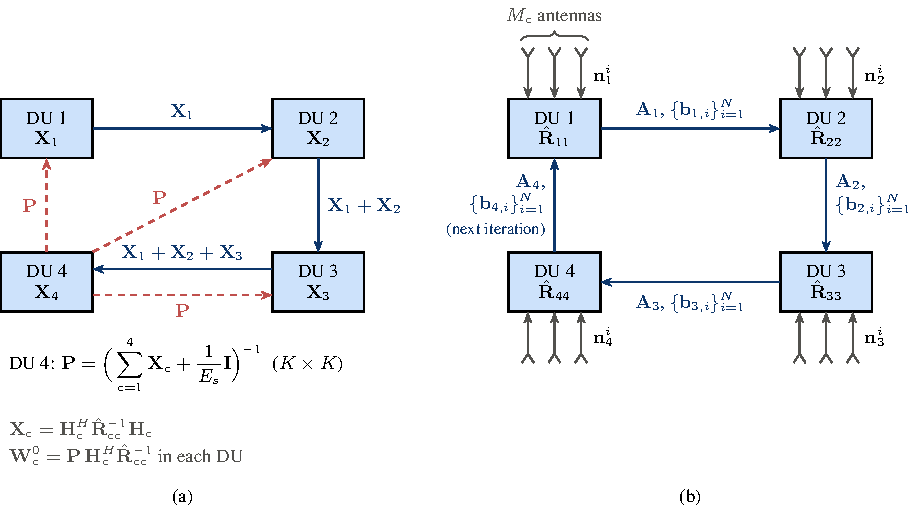
\includegraphics[width=\textwidth]{Images/FLUXO/bcd_etapas.pdf}
\vspace{4pt}
\legend{Source: adapted from \citesp{zhao2025jsac}.}
\end{figure}
% FONTE: figura de Images/FLUXO/src/bcd_etapas.tex. (a) zhao2025jsac paper.md:136-140 (Eq. 7);
%   modelo B, software/Restrições - Parâmetros.csv, linhas 56-65. (b) Algoritmo 3, paper.md:407-433 e :450.

The filter phase calculates $\tilde{\mathbf s}$ by \eqref{eq:bcd_filtro}.

% FONTE: zhao2025jsac paper.md: Eq. 7, :132-140; Algoritmo 3, :407-433; nota 6, :450; iterações, :449, :461 e :585.
%   Inversão K x K na última DU: software/Restrições - Parâmetros.csv, linhas 56-65 (modelo B).




% ---------------------------------------------------------------------
\subsection{Block Update}\label{subsec:bcd}
% ---------------------------------------------------------------------
DU $c$ updates its block in iteration $\mathrm{iter}$ as~\cite{zhao2021-globecom,zhao2025jsac}:
% FONTE: zhao2021-globecom L152 (Eq. 8, mesma inversa (E_s H_c H_c^H + R_cc)^-1).
\begin{multline}
  \mathbf{W}_c^{\mathrm{iter}} = \left(
    E_s \left(\mathbf{I}_K - \mathbf{A}_{c-1}^{\mathrm{iter}}
    + \mathbf{W}_c^{\mathrm{iter}-1}\mathbf{H}_c\right)\mathbf{H}_c^H
    - \frac{1}{N}\sum_{i=1}^{N}
      \left(\mathbf{b}_{c-1,i}^{\mathrm{iter}} - \mathbf{W}_c^{\mathrm{iter}-1}\mathbf{n}_c^i\right)
      \left(\mathbf{n}_c^i\right)^H
  \right) \\
  \times
  \underbrace{
    \left(E_s \mathbf{H}_c \mathbf{H}_c^H
    + \hat{\mathbf{R}}_{cc}\right)^{-1}
  }_{\text{local } M_c \times M_c \text{ inversion}},
  \label{eq:bcd_update}
\end{multline}
where $\mathbf{A}_{c-1}^{\mathrm{iter}} \in \mathbb{C}^{K \times K}$ and
$\{\mathbf{b}_{c-1,i}^{\mathrm{iter}} \in \mathbb{C}^{K \times 1}\}_{i=1}^{N}$
are interaction variables received from the previous DU, and
$\hat{\mathbf{R}}_{cc}$ is given by~\eqref{eq:Rcc_est}. After updating $\mathbf{W}_c^{\mathrm{iter}}$,
DU $c$ computes the updated interaction variables
\begin{align}
  \mathbf{A}_c^{\mathrm{iter}} &= \mathbf{A}_{c-1}^{\mathrm{iter}}
    - \mathbf{W}_c^{\mathrm{iter}-1}\mathbf{H}_c
    + \mathbf{W}_c^{\mathrm{iter}}\mathbf{H}_c, \label{eq:A_update} \\
  \mathbf{b}_{c,i}^{\mathrm{iter}} &= \mathbf{b}_{c-1,i}^{\mathrm{iter}}
    - \mathbf{W}_c^{\mathrm{iter}-1}\mathbf{n}_c^i
    + \mathbf{W}_c^{\mathrm{iter}}\mathbf{n}_c^i, \quad i = 1,\ldots,N,
  \label{eq:b_update}
\end{align}
and forwards them to DU $c+1$~\cite{zhao2025jsac}.

By~\eqref{eq:b_update}, $\mathbf b_{c,i}$ is the sum of $\mathbf W_j\mathbf n_j^i$ over all DUs $j$, where $\mathbf n_j^i$ is the $i$-th noise sample of cluster $j$. In the average of~\eqref{eq:bcd_update}, each term $\mathbf W_j\mathbf n_j^i(\mathbf n_c^i)^H$ results in $\mathbf W_j\hat{\mathbf R}_{jc}$. Thus, DU $c$ uses the off-diagonal blocks without estimating them (Figure~\ref{fig:rn-blocos}) \cite{zhao2025jsac}.
% FONTE: zhao2025jsac paper.md:447; Algoritmo 3 (b_0^0) e Eq. eq:b_update.
% FONTE (conta): (1/N) sum_i W_j n_j^i (n_c^i)^H = W_j R_jc.

$\mathbf G_c$ is the matrix inverted in~\eqref{eq:bcd_update}:
\begin{equation}\label{eq:Gc}
\mathbf G_c=
E_s\mathbf H_c\mathbf H_c^H+
\hat{\mathbf R}_{cc}.
\end{equation}
$\mathbf G_c$ does not depend on the iteration $\mathrm{iter}$ \cite{zhao2025jsac}. Thus, the DU inverts $\mathbf G_c$ once per coherence block and uses the inverse in all iterations.
% FONTE: Eq. 30, paper.md:504 (G_c sem índice de iteração).

% ---------------------------------------------------------------------
\subsection{Complexity}\label{subsubsec:bcd-complexidade}
% ---------------------------------------------------------------------

Preprocessing costs $\mathcal{O}(M_c^3 + N M_c^2)$ in each DU. Each iteration costs $\mathcal{O}(NMK + M M_c K)$ summed over all DUs \cite{zhao2025jsac}. The matrices of the algorithm have complex entries. Table~\ref{tab:bcd-complexidade} gives, for each part, the number of products between two complex numbers, called complex multiplications. Several parts depend on $N$, which changes with the test condition (Table~\ref{tab:n-maximo}).

\begin{table}[htbp]
\caption{Complex multiplications per PRB and per $T_c$ in each DU.}
\label{tab:bcd-complexidade}
\vspace{4pt}
\centering
\footnotesize
\renewcommand{\arraystretch}{1.2}
\setlength{\aboverulesep}{0pt}
\setlength{\belowrulesep}{0pt}
\begin{tabular}{|l|l|}
\toprule
\textbf{Part} & \textbf{Complex multiplications} \\
\midrule
Estimate $\hat{\mathbf R}_{cc}$ and apply Ledoit-Wolf & $N M_c^2 + N M_c + M_c^2$ \\
\hline
Initialization, including the inverse of $\hat{\mathbf R}_{cc}$ & $M_c^3 + M_c^2 K + M_c K^2 + 2K^2 M_c + N K M_c$ \\
\hline
Form $\mathbf G_c$ & $M_c^2 K$ \\
\hline
Invert $\mathbf G_c$ & $M_c^3$ \\
\hline
Each iteration & $2NKM_c + 3K^2 M_c + K M_c^2$ \\
\hline
Invert the $K \times K$ matrix (DU $C$ only) & $K^3$ \\
\hline
Filter, per data symbol & $12 K M_c$ \\
\bottomrule
\end{tabular}
\vspace{4pt}
\legend{Source: the author, from \citesp{zhao2025jsac}.}
\end{table}
% FONTE: software/Restrições - Parâmetros.csv, linhas 56-65 (modelo B); zhao2025jsac paper.md:136-142,
%   :410-418, :430-434, :443-449, :504, :554 e :556.
